%%\documentclass[a4paper,12pt,oneside]{llncs}
\documentclass{book}
%\usepackage[right=2cm,left=3cm,top=2cm,bottom=2cm,headsep=0cm]{geometry}

%%%%%%%%%%%%%%%%%%%%%%%%%%%%%%%%%%%%%%%%%%%%%%%%%%%%%%%%%%%
%% Juego de caracteres usado en el archivo fuente: UTF-8
\usepackage{ucs}
\usepackage[utf8x]{inputenc}
\usepackage{eurosym}

%%%%%%%%%%%%%%%%%%%%%%%%%%%%%%%%%%%%%%%%%%%%%%%%%%%%%%%%%%%
%% Juego de caracteres usado en la salida dvi
%% Otra posibilidad: \usepackage{t1enc}
\usepackage[T1]{fontenc}

%%%%%%%%%%%%%%%%%%%%%%%%%%%%%%%%%%%%%%%%%%%%%%%%%%%%%%%%%%%
%% Ajusta maergenes para a4
\usepackage{a4wide}

%%%%%%%%%%%%%%%%%%%%%%%%%%%%%%%%%%%%%%%%%%%%%%%%%%%%%%%%%%%
%% Uso fuente postscript times, para que los ps y pdf queden y pequeños...
\usepackage{times}

%%%%%%%%%%%%%%%%%%%%%%%%%%%%%%%%%%%%%%%%%%%%%%%%%%%%%%%%%%%
%% Posibilidad de hipertexto (especialmente en pdf)
\usepackage{hyperref}

%%%%%%%%%%%%%%%%%%%%%%%%%%%%%%%%%%%%%%%%%%%%%%%%%%%%%%%%%%%
%% Graficos 
\usepackage{graphics,graphicx}

%%%%%%%%%%%%%%%%%%%%%%%%%%%%%%%%%%%%%%%%%%%%%%%%%%%%%%%%%%%
%% Ciertos caracteres "raros"...
\usepackage{latexsym}

%%%%%%%%%%%%%%%%%%%%%%%%%%%%%%%%%%%%%%%%%%%%%%%%%%%%%%%%%%%
%% Matematicas aun más fuertes (american math dociety)
\usepackage{amsmath}

%%%%%%%%%%%%%%%%%%%%%%%%%%%%%%%%%%%%%%%%%%%%%%%%%%%%%%%%%%%
\usepackage{multirow} % para las tablas
\usepackage[spanish,es-tabla]{babel}

%%%%%%%%%%%%%%%%%%%%%%%%%%%%%%%%%%%%%%%%%%%%%%%%%%%%%%%%%%%
%% Fuentes matematicas lo mas compatibles posibles con postscript (times)
%% (Esto no funciona para todos los simbolos pero reduce mucho el tamaño del
%% pdf si hay muchas matamaticas....
\usepackage{mathptm}

%%% VARIOS:
%\usepackage{slashbox}
\usepackage{verbatim}
\usepackage{array}
\usepackage{listings}
\usepackage{multirow}
\usepackage{hhline}
\usepackage{titling}

%% MARCA DE AGUA
%% Este package de "draft copy" NO funciona con pdflatex
%%\usepackage{draftcopy}
%% Este package de "draft copy" SI funciona con pdflatex
%%%\usepackage{pdfdraftcopy}
%%%%%%%%%%%%%%%%%%%%%%%%%%%%%%%%%%%%%%%%%%%%%%%%%%%%%%%%%%%
%% Indenteacion en español...
\usepackage[spanish]{babel}
\usepackage{Estilos/Apuntes}
\usepackage[svgnames,x11names,table]{xcolor}
\usepackage{listingsutf8}
% Para escribir código en C
% \begin{verbatim}[language=C]
% #include <stdio.h>
% int main(int argc, char* argv[]) {
% puts("Hola mundo!");
% }
% \end{verbatim}
\usepackage{hyphenat}

\newenvironment{changemargin}[2]{%
	\begin{list}{}{%
			\setlength{\topsep}{0pt}%
			\setlength{\leftmargin}{#1}%
			\setlength{\rightmargin}{#2}%
			\setlength{\listparindent}{\parindent}%
			\setlength{\itemindent}{\parindent}%
			\setlength{\parsep}{\parskip}%
		}%
		\item[]}{\end{list}}
	
\newenvironment{nota}{
	\begin{changemargin}{2em}{2em}
		\textbf{\textsc{Nota: }}
	}{
	\end{changemargin}
}


\title{\huge{Fantasy}}
\author{Luis Gutiérrez Flores\\
	Nicolás Ruiz Requejo\\
	Jesús Rodríguez Heras\\
	Arantzazu Otal Alberro\\
	Alejandro Segovia Gallardo\\
	Alejandro José Caraballo García\\
	Gabriel Fernando Sánchez Reina}


%%Configuracion del paquete listings
\lstset{language=bash, numbers=left, numberstyle=\tiny, numbersep=10pt, firstnumber=1, stepnumber=1, basicstyle=\small\ttfamily, tabsize=1, extendedchars=true, inputencoding=utf8/latin1, breaklines=true}

\begin{document}
%	\maketitle

%	\begin{titlepage}
%		\centering
%		
%		{\scshape\huge Escuela Superior de Ingeniería \par}
%		\vspace{1cm}
%		{\scshape\LARGE Universidad de Cádiz\par}
%		\vspace{1cm}
%		{\scshape\Large{Stimey}\par}
%		\vspace{1cm}
%		{\Huge\bfseries Fantasy\par}
%		\vspace{1cm}
%		{\Large\itshape Luis Gutiérrez Flores\\
%			Nicolás Ruiz Requejo\\
%			Jesús Rodríguez Heras\\
%			Arantzazu Otal Alberro\\
%			Alejandro Segovia Gallardo\\
%			Alejandro José Caraballo García\\
%			Gabriel Fernando Sánchez Reina\par}
%		\vspace{2.5cm}
%		\begin{table}[htb]
%			\centering
%			\begin{tabular}{ccc}
%				
\includegraphics[width=0.15\textwidth]{UCA.png}\par\vspace{1.2cm} & 
\includegraphics[width=0.15\textwidth]{ESI.png}\par\vspace{1.2cm} & 
\includegraphics[width=0.15\textwidth]{Stimey.png}\par\vspace{1.2cm}
%			\end{tabular}
%		\end{table}
%%		\vfill
%		
%		
%		
%		% Bottom of the page
%%		{\large \today\par}
%	\end{titlepage}

\begin{titlepage}
	\centering
%	
\includegraphics[width=.1\textwidth]{UCA.png}

\begin{table}[htb]
				\centering
				\begin{tabular}{ccc}
					
\includegraphics[width=0.15\textwidth]{UCA.png}\par\vspace{0.2cm} & 
\includegraphics[width=0.15\textwidth]{ESI.png}\par\vspace{0.2cm} & 
\includegraphics[width=0.15\textwidth]{Stimey.png}\par\vspace{0.2cm}
				\end{tabular}
			\end{table}
	
%	\bigskip
%	\bigskip
%	\bigskip
	
	\begin{changemargin}{3em}{3em}
		\centering
		
		{\LARGE \textsc{\nohyphens{Escuela Superior de Ingeniería}}}
		
		\bigskip
		\bigskip
		\bigskip
		\bigskip
		
		{\LARGE \nohyphens{Grado en Ingeniería Informática}}
		
		\bigskip
		\bigskip
%		\bigskip
		\bigskip
		\bigskip
		\bigskip
		
		{\LARGE \nohyphens{\textbf{Fantasy}}}
		
		\bigskip
		\bigskip
%		\bigskip
		\bigskip
		\bigskip
		
		{\large Curso 2018-2019}
		
		\bigskip
		\bigskip
%		\bigskip
%		\bigskip
		\bigskip
		\bigskip
		
	\end{changemargin}
	
	{\Large Luis Gutiérrez Flores\\
					Nicolás Ruiz Requejo\\
					Jesús Rodríguez Heras\\
					Arantzazu Otal Alberro\\
					Alejandro Segovia Gallardo\\
					Alejandro José Caraballo García\\
					Gabriel Fernando Sánchez Reina} \\
	\bigskip
	\bigskip 
	\bigskip 
	{\large Puerto Real, \today}
	
\end{titlepage}
\newpage{\pagestyle{empty}\cleardoublepage}  
{
	\thispagestyle{empty} 
	\centering
%	
\includegraphics[width=.1\textwidth]{UCA.png}
\begin{table}[htb]
	\centering
	\begin{tabular}{ccc}
		
\includegraphics[width=0.15\textwidth]{UCA.png}\par\vspace{0.2cm} & 
\includegraphics[width=0.15\textwidth]{ESI.png}\par\vspace{0.2cm} & 
\includegraphics[width=0.15\textwidth]{Stimey.png}\par\vspace{0.2cm}
	\end{tabular}
\end{table}
	
%	\bigskip
%	\bigskip
%	\bigskip
	
	\begin{changemargin}{3em}{3em}
		
		\begin{center}
			{\LARGE \textsc{\nohyphens{Escuela Superior de Ingeniería}}}
			
			\bigskip
			\bigskip
			
			{\LARGE \nohyphens{Grado en Ingeniería Informática}}
			
			\bigskip
			\bigskip
			\bigskip
			\bigskip
			
			{\LARGE \nohyphens{\textbf{Fantasy}}}
			
			\bigskip
			\bigskip
			\bigskip
			\bigskip
			
		\end{center}
	\end{changemargin}
	
	\begin{flushleft}
		\Large
		
		\textsc{Departamento}: \nohyphens{Ingeniería Informática.} \\
		\textsc{Directora del proyecto}: \nohyphens{Alicia Ale.} \\
		\textsc{Autor del Proyecto}: \nohyphens{Equipo Fantasy}. \\
	\end{flushleft}
	
	\bigskip
	\bigskip
	\bigskip
	
	\begin{flushright}
		\large
		Puerto Real, \today
		
		\bigskip    
		\bigskip
		\bigskip
		\bigskip
		\bigskip
		\bigskip
		\bigskip
		\bigskip
		Fdo.: Equipo Fantasy
		
	\end{flushright}
	
}
	
%	\thispagestyle{empty}
	\newpage
	
	\newpage{\pagestyle{empty}\cleardoublepage} 
\vspace*{\fill}
\begin{center}
	\textbf{Resumen}
\end{center}
Aplicación web para fomentar el aprendizaje mediante la imaginación y creatividad de niños entre 10 y 13 años en temas científicos-tecnológicos en colaboración con el proyecto europeo STIMEY.

A modo de juego, los niños podrán crear historias interactivas y los profesores podrán evaluarlos.\\

\textbf{Palabras clave:}
Fantasía, aprendizaje, desarrollo, ilusiona, entretenimiento, creatividad, cuestionario, evalua-
ción, enseñanza, ciencia, unión europea.
\vspace*{\fill}

\newpage

	
	\tableofcontents
	\newpage
	
	\part{Prolegómeno}
	\chapter{Introducción}
\section{Motivación}
Es un trabajo de la asignatura ``Proyectos Informáticos'' que, a nivel profesional, nos sirve para ganar experiencia laboral y enfrentarnos a situaciones reales de cara a una clientela exigente.

\section{Descripción del sistema actual}
Inicialmente, nuestra clienta contaba con una aplicación que mostraba en una página la información a cerca de un tema y los alumnos no se centraban en aprender, sino que iban directamente a hacer el cuestionario final con el objetivo de terminar antes. Esto hace que los alumnos no aprendan como es debido ni fomenten su imaginación ni su creatividad.

\section{Objetivos y alcance del proyecto}
\subsection{Objetivos}
Motivación de la creatividad y fomento de la imaginación en niños.

Para cumplir con el objetivo general, tendremos que cubrir los siguientes puntos:
\begin{itemize}
	\item Recursos de aprendizaje interactivos.
	\item Es evaluable por un profesor.
	\item Se pueden compartir fantasías entre usuarios.
	\item Es simple y manejable por alumnos de primaria.
	\item Fomenta las habilidades y enseñanzas STEM (science, technology, engeneering and maths).
\end{itemize}

\subsection{Alcance}
Los alumnos podrán crear fantasías, compartirlas y podrán ser evaluadas por los profesores, que podrán mandar como tarea el hacer fantasías.

\section{Organización del documento}
Este documento está organizado en función de las especificaciones expuestas para la presentación de un trabajo de fin de grado siguiendo los siguientes apartados:
\begin{enumerate}
	\item Introducción.
	\item Plan de proyecto.
	\item Análisis de requisitos.
	\item Diseño del sistema.
	\item Implementación del sistema.
	\item Pruebas del sistema.
	\item Manual de usuario.
	\item Manual de instalación.
	\item Conclusiones.
\end{enumerate}

Además de este documento, también contamos con un apéndice donde se narra el manual de usuario, paso a paso.

	\chapter{Planificación}
En este capítulo se recoge la planificación, el planteamiento y el principio de un proyecto al que hemos denominado ``\textbf{Fantasy}'', un portal web en el que los profesores pueden realizar una serie de tareas (fantasías) con el objetivo de que los alumnos puedan jugarlas y así aprendan de forma creativa.

Los alumnos, también tendrán la posibilidad de crear las fantasías que el profesor les mande como trabajo y luego serán evaluadas por dicho profesor.

\section{Metodología de desarrollo}
La metodología usada será \textbf{Scrum}: Método de desarrollo ágil caracterizado por tener un desarrollo incremental y basar la calidad del resultado en el conocimiento más que en los procesos empleados.

\section{Planificación del proyecto}
El proyecto tendrá una duración de tres meses y se realizarán reuniones semanales con el cliente de una hora de duración como máximo.
\begin{figure}[h]
	\centering
	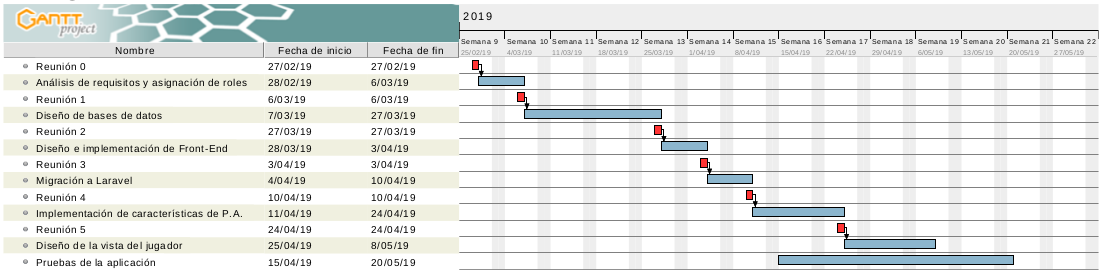
\includegraphics[scale=0.42]{Gantt.png}
	\caption{Diagrama de Gantt}
	\label{Diagrama de Gantt}
\end{figure}

\section{Organización}
\subsection{Roles}
\begin{itemize}
	\item \textbf{Administrador:} Luis Gutiérrez Flores.
	\item \textbf{Analistas:} Jesús Rodríguez Heras y Nicolás Ruiz Requejo.
	\item \textbf{Diseñadores:} Arantzazu Otal Alberro, Gabriel Fernando Sánchez Reina y Nicolás Ruiz Requejo.
	\item \textbf{Desarrolladores:} Luis Gutiérrez Flores, Alejandro Segovia Gallardo y Alejandro José Caraballo García.
	\item \textbf{Ingenieros de pruebas:} Jesús Rodríguez Heras y Luis Gutiérrez Flores.
\end{itemize}

\subsection{Recursos hardware y software}
Como recursos hardware tenemos los portátiles de los 7 miembros del grupo y el servidor de Stimey.

Como recursos software tenemos el framework Laravel, Atom, Visual Studio Code, TeXStudio, PhPMyAdmin, MySQL, GitHub.

\section{Costes}
\subsection{Costes humanos}
\begin{itemize}
	\item Horas en el aprendizaje de Laravel.
	\item Horas en formación de PHP y MySQL.
	\item Horas en formación de GitHub.
	\item Horas de documentación.
\end{itemize}

\subsection{Costes materiales}
\begin{itemize}
	\item Nuestros ordenadores.
	\item Transporte a la escuela.
	\item Gastos del servidor de Stimey.
\end{itemize}

\section{Gestión de riesgos}
\begin{itemize}
	\item No cumplir plazos por intentar abarcar demasiado y dejar funcionalidades incompletas.
\end{itemize}

\section{Política de equipo}
El equipo ha decidido hacer reuniones con una periodicidad de una semana con el cliente, a lo largo de la semana, los integrantes del equipo intentarán establecer reuniones entre ellos con la duración necesaria para continuar avanzando en el proyecto (tiempo estimado: dos horas).

\section{Hitos} %Seguir poniendo los demás sprints
\subsection{Sprint 0 (27 de febrero al 6 de marzo)}
\begin{enumerate}
	\item Creación de plataformas de trabajo y control de versiones (GitHub).
	\item Creación del boceto de requisitos.
	\item Creación de casos de uso y sus descripciones.
\end{enumerate}
\subsection{Sprint 1 (6 de marzo al 27 de marzo)}
\begin{enumerate}
	\item Creación de mockups de la plataforma.
	\item Implementación de la base de datos.
\end{enumerate}

\subsection{Sprint 2 (27 de marzo al 3 de abril)}
\begin{enumerate}
	\item Implementación de front-end.
	\item Migraciones de la base de datos.
	\item Adaptación del proyecto al framework Laravel.
	\item Creación de fantasías.
\end{enumerate}

\subsection{Sprint 3 (3 de abril al 10 de abril)}
\begin{enumerate}
	\item Finalización de front-end.
	\item Migraciones finales de la base de datos.
	\item Finalización de la creación de fantasías.
\end{enumerate}

\subsection{Sprint 4 (10 de abril al 24 de abril)}
\begin{enumerate}
	\item Finalización de las migraciones de la base de datos.
	\item Creación de puntos activos con sus características básicas.
\end{enumerate}

\subsection{Sprint 5 (24 de abril al 1 de mayo)}
\begin{enumerate}
	\item Creación de puntos activos con todas sus características.
	\item Inicio de la vista para poder jugar la fantasía.
\end{enumerate}


\section{Reuniones}
\subsection{Reunión 0 (27 de febrero)}
\begin{enumerate}
	\item Análisis de requisitos del sistema.
	\item Creación de casos de uso.
	\item Planteamiento de la base de datos del sistema.
	\item Distribución de las tareas del sprint 0.
\end{enumerate}

\subsection{Reunión 1 (6 de marzo)}
\begin{enumerate}
	\item Finalización del sprint 0.
	\item Distribución de la información a buscar.
	\item Comienzo del sprint 1.
\end{enumerate}

\subsection{Reunión 2 (27 de marzo)}
\begin{enumerate}
	\item Finalización del sprint 1.
	\item Comienzo del sprint 2.
\end{enumerate}

\subsection{Reunión 3 (3 de abril)}
\begin{enumerate}
	\item Finalización del sprint 2.
	\item Comienzo del sprint 3.
\end{enumerate}

\subsection{Reunión 4 (10 de abril)}
\begin{enumerate}
	\item Finalización del sprint 3.
	\item Comienzo del sprint 4.
\end{enumerate}

\subsection{Reunión 5 (24 de abril)}
\begin{enumerate}
	\item Finalización del sprint 4.
	\item Comienzo del sprint 5.
\end{enumerate}

	
	\part{Desarrollo}
	\chapter{Análisis de requisitos}
\section{Workspace}
El diseño gráfico usado deberá ser el mismo que el de la página de Stimey en todos los iconos usados: \url{https://stimey.eu/home}. Si necesitamos algo más, Alicia, nos lo podría facilitar.

El profesor tendrá más permisos y privilegios que el alumno, de forma que pueda crear fantasías para evaluar a sus alumnos y ellos tendrán que completarlas o crear las que el profesor les ponga como trabajo.

En el workspace tendremos una serie de opciones que estarán disponibles tanto para el rol de profesor como de alumno en función de los permisos de cada rol:
\begin{itemize}
	\item \textbf{Background:} Se abre una ventana donde se podrá seleccionar una imagen usada anteriormente, de google o del ordenador. Esta imagen cubrirá todo el workspace. También será posible introducir texto añadiéndolo manualmente o mediante un link.
	\item \textbf{Punto Activo:} Establece un punto activo en el workspace (arrastrando y soltando).
	\begin{itemize}
		\item Será posible moverlo y modificar los contenidos del mismo.
		\item Si se añade una imagen al puto activo, dicho punto, se adapta a la forma de la imagen.
		\item Una vez originado el punto activo se abre un pop\_up con un texto.
		\item También se puede asignar un vídeo, que abrirá una ventana para reproducirlo, o un audio. En caso de que no exista audio o vídeo, no se mostrará el respectivo botón.
		\item Los puntos activos podrán tener música de fondo que será silenciada si se inicia la reproducción de audio o vídeo asignados a dicho punto por el profesorado. La música será restablecida al terminar el audio o vídeo correspondiente.
		\item Los puntos activos pueden ser reorganizados por el profesorado para que emerjan en el orden que ellos quieran.
		\item Un alumno no puede continuar con el siguiente punto activo sin terminar el actual.
		\item El quiz de los puntos activos debe ser divertido.
		\item Las cuestiones planteadas en los quiz de los puntos activos deberán ser 2 y no demasiado difíciles (respuesta múltiple, escribir una palabra, quiz con imágenes y preguntas sobre ésta, unir items, etc).
		\item El quiz saldrá en pantalla cuando se cierra el punto activo actual.
		\item Una vez acabado el quiz, aparece el siguiente punto activo en el orden establecido por el profesorado en el workspace.
		\item Cada punto activo tendrá una puntuación hasta sumar entre todos un máximo de 100 puntos.
		\item Al asignar una puntuación a un punto activo, ésta se restará al total que llevemos (máximo 100 puntos). Si un punto activo es eliminado, el contador general recupera la puntuación que tenía asignada dicho punto activo.
		\item El alumno no sabe el total de puntos activos que hay en total.
		\item Cuando el alumno obtiene una puntuación al completar un punto activo, dicha cantidad se suma al contador global.
		\item Finalmente, podremos tener un resumen estadístico con las preguntas acertadas/falladas de cada punto activo.
		\item Solo se guardará la puntuación obtenida la primera vez que se realice un quiz, luego, se podrán hacer más veces, pero la nota no se registrará.
		\item El alumno tendrá la opción de guardar su progreso con un botón de guardar manualmente o mediante la opción de autoguardado.
	\end{itemize}
\end{itemize}

\section{Características}
\begin{itemize}
	\item Al finalizar todos los puntos activos habrá un botón abajo a la derecha de ``\textbf{más información}'' y en el centro un nuevo quiz que será el examen final. Este examen tendrá una puntuación independiente al de todos los puntos activos y no tendrá el resumen estadístico. Si se repite este quiz, la nota del mismo se actualizaría con un tanto por ciento de la nueva nota, más la nota anterior con el objetivo de que un alumno que repita un quiz no pueda obtener la mejor nota por repetición del mismo.
	\item El profesorado podrá mandar a los alumnos hacer fantasías para aprender como tarea. Estas tareas podrán realizarse en grupos de alumnos en función de dos ideas:
	\begin{enumerate}
		\item \textbf{Obligatoria:} Un alumno realiza la fantasía y el resto busca información adicional.
		\item \textbf{Opcional pero ideal:} Edición concurrente de la fantasía entre todos los integrantes del grupo.
	\end{enumerate}
	\item Cada fantasía tendrá un código para poder ser compartida.
	\item Tendremos dos tipos de permisos en las fantasías: ``\textbf{ver}'' y ``\textbf{ver y editar}''.
	\item La plataforma notificará al profesorado cuando los alumnos hayan terminado sus respectivos trabajos.
	\item Las fantasías podrán ser privadas o públicas. Por defecto, siempre serán públicas y podrán ser accedidas por todo el que utilice la plataforma.
	\item Las fantasías privadas podrán ser accedidas por otras personas mediante una contraseña.
	\item Las fantasías podrán ser clonadas.
\end{itemize}

	\chapter{Diseño del sistema}
%
% Se supone que debería quitar los que se parecen para que quede más corto la cosa es saber cual quitar y cual dejar.
%
\section{Diseño de casos de uso}
En el diseño del sistema se han propuesto una serie de casos de uso que tienen la siguiente precondición implícita para poder usar dichos casos de uso en la aplicación final:
\begin{itemize}
	\item El usuario (profesorado/alumnado) debe tener una cuenta en la plataforma de STIMEY y haber iniciado sesión con dicha cuenta.
\end{itemize}

Los casos de uso propuestos son los siguientes:

\subsection{CRUD fantasía}
\hypertarget{crearfantasia}{}
\subsubsection{Caso de uso: Crear fantasía}
\begin{itemize}
	\item \textbf{Descripción:} Crea una nueva fantasía.
	\item \textbf{Actores:} Creador-editor (usuario).
	\item \textbf{Precondiciones:} El usuario debe tener permisos para crear una nueva fantasía.
	\item \textbf{Postcondiciones:} La fantasía queda almacenada en el sistema.
	\item \textbf{Escenario principal:}
	\begin{enumerate}
		\item El usuario selecciona la opción ``Crear nueva fantasía''.
		\item El sistema solicita el nombre de la fantasía.
		\item El usuario introduce el nombre de la fantasía.
		\item El sistema solicita el código de la fantasía.
		\item El usuario introduce el código de la fantasía.
		\item El sistema da a elegir si la fantasía será pública (por defecto), compartida o privada.
		\item El usuario selecciona ``Pública''.
		\item El usuario crea la fantasía.
		\item La fantasía queda almacenada en el sistema.
	\end{enumerate}
	\item \textbf{Extensiones:} \\7. a) El usuario selecciona que la fantasía será compartida.
	\begin{enumerate}
		\item El sistema permite insertar en una lista los identificadores de otros usuarios con los que quedará compartida la fantasía.
		\item El usuario introduce los identificadores de los usuarios que compartirán la fantasía.
		\item Paso 8.
	\end{enumerate}
	7. b) El usuario selecciona que la fantasía será privada.
	\begin{enumerate}
		\item El sistema marca la fantasía como privada para dicho usuario sin dar la posibilidad de compartir.
		\item Paso 8.
	\end{enumerate}
	*a) En cualquier momento, el usuario puede volver atrás al menú principal.
	\item \textbf{Variaciones:} Ninguna.
	\item \textbf{No-funcional:} Ninguna.
	\item \textbf{Cuestiones:} Ninguna.
\end{itemize}

\subsubsection{Caso de uso: Visualizar fantasía}
\begin{itemize}
	\item \textbf{Descripción:} Lee una fantasía ya existente.
	\item \textbf{Actores:} Creador-editor (usuario).
	\item \textbf{Precondiciones:} La fantasía debe existir en el sistema y el usuario debe tener permisos de modificación.
	\item \textbf{Postcondiciones:} No se producen cambios en la fantasía.
	\item \textbf{Escenario principal:}
	\begin{enumerate}
		\item El usuario selecciona la opción ``Mis fantasías''
		\item El sistema muestra una lista de las fantasías accesibles por el usuario.
		\item El usuario selecciona la fantasía que desea visualizar.
		\item El sistema muestra una ventana emergente con la información de la fantasía y sus opciones.
		\item El usuario selecciona la opción ``Visualizar fantasía''.
		\item El sistema muestra la fantasía.
		\item El usuario lee la fantasía sin hacer ningún cambio y, cuando acaba, cierra la fantasía.
		\item La fantasía queda sin modificar.
	\end{enumerate}
	\item \textbf{Extensiones:} \\ *a) En cualquier momento, el usuario puede volver atrás al menú principal.
	\item \textbf{Variaciones:} Ninguna.
	\item \textbf{No-funcional:} Ninguna.
	\item \textbf{Cuestiones:} Ninguna.
\end{itemize}

\subsubsection{Caso de uso: Modificar fantasía}
\begin{itemize}
	\item \textbf{Descripción:} Modifica una fantasía ya existente.
	\item \textbf{Actores:} Creador-editor (usuario).
	\item \textbf{Precondiciones:} La fantasía debe existir en el sistema y el usuario debe tener permisos de modificación.
	\item \textbf{Postcondiciones:} La fantasía queda modificada.
	\item \textbf{Escenario principal:}
	\begin{enumerate}
		\item El usuario selecciona la opción ``Mis fantasías''.
		\item El sistema muestra una lista de las fantasías accesibles por el usuario.
		\item El usuario selecciona la fantasía que desea modificar.
		\item El sistema muestra una ventana emergente con la información de la fantasía y sus opciones.
		\item El usuario selecciona la opción ``Modificar fantasía''.
		\item El sistema muestra la pantalla de creación de la fantasía para su modificación.
	\end{enumerate}
	\item \textbf{Extensiones:} \\ *a) En cualquier momento, el usuario puede volver atrás al menú principal.
	\item \textbf{Variaciones:} Ninguna.
	\item \textbf{No-funcional:} Ninguna.
	\item \textbf{Cuestiones:} Ninguna.
\end{itemize}

\subsubsection{Caso de uso: Borrar fantasía}
\begin{itemize}
	\item \textbf{Descripción:} Borra una fantasía ya existente.
	\item \textbf{Actores:} Creador-editor (usuario).
	\item \textbf{Precondiciones:} La fantasía debe existir en el sistema y el usuario debe tener permisos de eliminación.
	\item \textbf{Postcondiciones:} La fantasía es eliminada del sistema.
	\item \textbf{Escenario principal:}
	\begin{enumerate}
		\item El usuario selecciona la opción ``Mis fantasías''.
		\item El sistema muestra una lista de las fantasías accesibles por el usuario.
		\item El usuario selecciona la fantasía que desea modificar.
		\item El sistema muestra una ventana emergente con la información de la fantasía y sus opciones.
		\item El usuario selecciona la opción ``Borrar fantasía''.
		\item El sistema muestra un mensaje de confirmación.
		\item El usuario selecciona ``Aceptar''.
		\item El sistema borra la fantasía.
	\end{enumerate}
	\item \textbf{Extensiones:}  \\7. a) El usuario selecciona ``Cancelar''.
	\begin{enumerate}
		\item El sistema cierra la ventana emergente.
		\item Paso 1.
	\end{enumerate}
	*a) En cualquier momento, el usuario puede volver atrás al menú principal.
	\item \textbf{Variaciones:} Ninguna.
	\item \textbf{No-funcional:} Ninguna.
	\item \textbf{Cuestiones:} Ninguna.
\end{itemize}


\subsection{Caso de uso: Elegir idioma}
\begin{itemize}
	\item \textbf{Descripción:} Cambia el idioma de la aplicación.
	\item \textbf{Actores:} Profesor o alumno (usuario).
	\item \textbf{Precondiciones:} Ninguna. %el usuario es capaz de encontrar el menú de idioma con la mirada
	\item \textbf{Postcondiciones:} La aplicación cambia al idioma seleccionado por el usuario.
	\item \textbf{Escenario principal:}
	\begin{enumerate}
		\item El usuario pulsa el botón de cambio de idioma.
		\item El sistema despliega una lista de los idiomas disponibles.
		\item El usuario  selecciona un idioma de los que están disponibles en el sistema.
		\item La aplicación cambia el idioma.
	\end{enumerate}
	\item \textbf{Extensiones:} Ninguna.
	\item \textbf{Variaciones:} Ninguna.
	\item \textbf{No-funcional:} Ninguna.
	\item \textbf{Cuestiones:} Ninguna.
\end{itemize}

\subsection{Caso de uso: Copiar fantasía}
\begin{itemize}
	\item \textbf{Descripción:} Clona una fantasía.
	\item \textbf{Actores:} Creador-editor (usuario).
	\item \textbf{Precondiciones:} La fantasía debe existir en el sistema y el usuario debe tener permisos de modificación.
	\item \textbf{Postcondiciones:} Crea una copia de la fantasía seleccionada.
	\item \textbf{Escenario principal:}
	\begin{enumerate}
		\item El usuario selecciona la opción ``Mis fantasías''.
		\item El sistema muestra una lista de las fantasías accesibles por el usuario.
		\item El usuario selecciona la fantasía que desea copiar.
		\item El sistema muestra una ventana emergente con la información de la fantasía y sus opciones.
		\item El usuario selecciona la opción ``Copiar fantasía''.
		\item El sistema crea una copia de la fantasía seleccionada.
	\end{enumerate}
	\item \textbf{Extensiones:} \\ *a) En cualquier momento, el usuario puede volver atrás al menú principal.
	\item \textbf{Variaciones:} Ninguna.
	\item \textbf{No-funcional:} Ninguna.
	\item \textbf{Cuestiones:} Ninguna.
\end{itemize}

\subsection{CRUD background}
\begin{itemize}
	\item \textbf{Descripción:} Permite seleccionar, modificar y borrar el background.
	\item \textbf{Actores:} Creador-editor (usuario).
	\item \textbf{Precondiciones:} La fantasía debe existir en el sistema y el usuario debe tener permisos de modificación.
	\item \textbf{Postcondiciones:} Se establece el fondo que el usuario haya elegido.
	\item \textbf{Escenario principal:}
	\begin{enumerate}
		\item El usuario selecciona la opción ``Background``.
		\item El sistema muestra una ventana para añadir un background al workspace.
		\item El usuario selecciona una imagen. %puede ser un color
		\item El sistema establece el background seleccionado por el usuario.
	\end{enumerate}
	\item \textbf{Extensiones:} \\ *a) En cualquier momento, el usuario puede volver atrás al menú principal. 
	\item \textbf{Variaciones:} Ninguna.
	\item \textbf{No-funcional:} Ninguna.
	\item \textbf{Cuestiones:} Ninguna.
\end{itemize}


\subsection{CRUD punto activo}
\subsubsection{Caso de uso: Crear punto activo}
\begin{itemize}
	\item \textbf{Descripción:} Crea un punto activo nuevo.
	\item \textbf{Actores:} Creador-editor (usuario).
	\item \textbf{Precondiciones:} La fantasía debe existir en el sistema y el usuario debe tener permisos de modificación.
	\item \textbf{Postcondiciones:} Se crea un punto activo vacío en el workspace.
	\item \textbf{Escenario principal:}
	\begin{enumerate}
		\item El usuario selecciona la opción ``Nuevo punto activo''.
		\item El sistema crea un nuevo punto activo en el workspace.
		\item El usuario puede mover el punto activo a la zona del workspace que desee.
		\item El sistema guardará el punto activo en la fantasía.
	\end{enumerate}
	\item \textbf{Extensiones:} \\ *a) En cualquier momento, el usuario puede volver atrás.
	\item \textbf{Variaciones:} Ninguna.
	\item \textbf{No-funcional:} Ninguna.
	\item \textbf{Cuestiones:} Ninguna.
\end{itemize}

\subsubsection{Caso de uso: Visualizar punto activo}
\begin{itemize}
	\item \textbf{Descripción:} Muestra un punto activo existente para su lectura.
	\item \textbf{Actores:} Creador-editor (usuario).
	\item \textbf{Precondiciones:} La fantasía debe existir en el sistema y el punto activo debe existir en la fantasía. Además, el usuario debe tener permisos de modificación.
	\item \textbf{Postcondiciones:} Se muestra el punto activo para su lectura.
	\item \textbf{Escenario principal:}
	\begin{enumerate}
		\item El usuario selecciona el punto activo que desea visualizar.
		\item El sistema muestra una ventana con la información del punto activo y sus opciones.
		\item El usuario selecciona la opción ``Visualizar''.
		\item El sistema muestra una ventana con el resumen de dicho punto activo.
	\end{enumerate}
	\item \textbf{Extensiones:} \\ *a) En cualquier momento, el usuario puede volver atrás.
	\item \textbf{Variaciones:} Ninguna.
	\item \textbf{No-funcional:} Ninguna.
	\item \textbf{Cuestiones:} Ninguna.
\end{itemize}

\subsubsection{Caso de uso: Modificar punto activo}
\begin{itemize}
	\item \textbf{Descripción:} Modifica un punto activo existente.
	\item \textbf{Actores:} Creador-editor (usuario).
	\item \textbf{Precondiciones:} La fantasía debe existir en el sistema y el punto activo debe existir en la fantasía. Además, el usuario debe tener permisos de modificación.
	\item \textbf{Postcondiciones:} Modifica el punto activo seleccionado.
	\item \textbf{Escenario principal:}
	\begin{enumerate}
		\item El usuario selecciona el punto activo que desea modificar.
		\item El sistema muestra una ventana con la información del punto activo y sus opciones.
		\item El usuario selecciona la opción ``Modificar''.
		\item El sistema muestra la ventana de creación del punto activo.
	\end{enumerate}
	\item \textbf{Extensiones:} \\ *a) En cualquier momento, el usuario puede volver atrás.
	\item \textbf{Variaciones:} Ninguna.
	\item \textbf{No-funcional:} Ninguna.
	\item \textbf{Cuestiones:} Ninguna.
\end{itemize}

\subsubsection{Caso de uso: Borrar punto activo}
\begin{itemize}
	\item \textbf{Descripción:} Borra un punto activo existente.
	\item \textbf{Actores:} Creador-editor (usuario).
	\item \textbf{Precondiciones:} La fantasía debe existir en el sistema y el punto activo debe existir en la fantasía. Además, el usuario debe tener permisos de modificación.
	\item \textbf{Postcondiciones:} Borra el punto activo seleccionado.
	\item \textbf{Escenario principal:}
	\begin{enumerate}
		\item El usuario selecciona el punto activo que desea eliminar.
		\item El sistema muestra una ventana con la información del punto activo y sus opciones.
		\item El usuario selecciona la opción ``Borrar''.
		\item El sistema muestra un mensaje de confirmación.
		\item El usuario selecciona ``Aceptar''.
		\item El sistema borra el punto activo.
	\end{enumerate}
	\item \textbf{Extensiones:} \\ 5. a) El usuario selecciona ``Cancelar''.
	\begin{enumerate}
		\item El sistema cierra la ventana emergente.
		\item Paso 1.
	\end{enumerate}
	*a) En cualquier momento, el usuario puede volver atrás.
	\item \textbf{Variaciones:} Ninguna.
	\item \textbf{No-funcional:} Ninguna.
	\item \textbf{Cuestiones:} Ninguna.
\end{itemize}

\subsection{CRUD imagen} %suponemos que es para un punto activo
\hypertarget{crearimagen}{}
\subsubsection{Caso de uso: Crear imagen}
\begin{itemize}
	\item \textbf{Descripción:} Inserta una imagen en un punto activo.
	\item \textbf{Actores:} Creador-editor (usuario).
	\item \textbf{Precondiciones:} Debe existir el punto activo correspondiente y se debe estar editando la fantasía.
	\item \textbf{Postcondiciones:} Inserta una imagen en el punto activo seleccionado.
	\item \textbf{Escenario principal:}
	\begin{enumerate}
		\item El usuario selecciona el punto activo correspondiente dentro de la fantasía.
		\item El sistema muestra una ventana emergente con la información del punto activo.
		\item El usuario selecciona la opción de ``Insertar imagen''.
		\item El sistema muestra una ventana en la que da a elegir al usuario de dónde quiere seleccionar la imagen (Internet, local, imagen ya usada en la fantasía).
		\item El usuario elige la opción ``Internet'' para incluir una imagen de Internet.
		\item El sistema le pide al usuario la url de la imagen.
		\item El usuario inserta la url correcta de la imagen.
		\item El punto activo toma la forma de la imagen.
	\end{enumerate}
	\item \textbf{Extensiones:} \\5. a) El usuario elige la opción ``Local'' para incluir una imagen desde su ordenador.
	\begin{enumerate}
		\item El sistema abre una ventana del explorador de archivos.
		\item El usuario selecciona la imagen deseada y pulsa ``Aceptar''.
		\item El sistema cierra la ventana del explorador de archivos.
		\item Paso 8.
	\end{enumerate}
	5. b) El usuario elige la opción ``Imagen usada anteriormente'' para incluir una imagen ya usada.
	\begin{enumerate}
		\item El sistema abre una ventana con las imágenes usadas anteriormente.
		\item El usuario selecciona la imagen deseada y pulsa ``Aceptar''.
		\item El sistema cierra la ventana emergente.
		\item Paso 8.
	\end{enumerate}
	7. a) La url no es correcta.
	\begin{enumerate}
		\item El sistema muestra un mensaje de error.
		\item Paso 6.
	\end{enumerate}
	*a) En cualquier momento, el usuario puede volver atrás.
	\item \textbf{Variaciones:} Ninguna.
	\item \textbf{No-funcional:} Ninguna.
	\item \textbf{Cuestiones:} ¿Podrá modificar el tamaño original de la imagen o hacer recortes?
\end{itemize}

\subsubsection{Caso de uso: Modificar imagen}
\begin{itemize}
	\item \textbf{Descripción:} Modifica una imagen.
	\item \textbf{Actores:} Creador-editor (usuario).
	\item \textbf{Precondiciones:} Debe existir el punto activo correspondiente, se debe estar editando la fantasía y debe existir una imagen.
	\item \textbf{Postcondiciones:} La imagen queda modificada.
	\item \textbf{Escenario principal:}
	\begin{enumerate}
		\item El usuario selecciona el punto activo correspondiente dentro de la fantasía.
		\item El sistema abre una ventana emergente con la información del punto activo.
		\item Paso 4 de \hyperlink{crearimagen}{Crear imagen}.
	\end{enumerate}
	\item \textbf{Extensiones:} \\ *a) En cualquier momento, el usuario puede volver atrás.
	\item \textbf{Variaciones:} Ninguna.
	\item \textbf{No-funcional:} Ninguna.
	\item \textbf{Cuestiones:} Ninguna.
\end{itemize}

\subsubsection{Caso de uso: Borrar imagen}
\begin{itemize}
	\item \textbf{Descripción:} Borra una imagen de un punto activo.
	\item \textbf{Actores:} Creador-editor (usuario).
	\item \textbf{Precondiciones:} Debe existir el punto activo correspondiente, se debe estar editando la fantasía y debe existir una imagen.
	\item \textbf{Postcondiciones:} Borra la imagen y deja el punto activo en su estado por defecto.
	\item \textbf{Escenario principal:}
	\begin{enumerate}
		\item El usuario selecciona el punto activo correspondiente dentro de la fantasía.
		\item El sistema abre una ventana emergente con la información del punto activo.
		\item El usuario selecciona la imagen y pulsa el botón ``Suprimir''.
		\item El sistema muestra un mensaje de confirmación.
		\item El usuario selecciona ``Aceptar''.
		\item El sistema borra la imagen del punto activo.
	\end{enumerate}
	\item \textbf{Extensiones:} \\ 5. a) El usuario selecciona ``Cancelar''.
	\begin{enumerate}
		\item El sistema cierra la ventana emergente.
		\item Paso 1.
	\end{enumerate}
	*a) En cualquier momento, el usuario puede volver atrás.
	\item \textbf{Variaciones:} Ninguna.
	\item \textbf{No-funcional:} Ninguna.
	\item \textbf{Cuestiones:} Ninguna.
\end{itemize}

\subsection{CRUD vídeo}
\hypertarget{crearvideo}{}
\subsubsection{Caso de uso: Crear vídeo}
\begin{itemize}
	\item \textbf{Descripción:} Inserta un vídeo dentro de un punto activo.
	\item \textbf{Actores:} Creador-editor (usuario).
	\item \textbf{Precondiciones:} Debe existir el punto activo correspondiente y se debe estar editando la fantasía.
	\item \textbf{Postcondiciones:} Inserta un vídeo en el punto activo seleccionado.
	\item \textbf{Escenario principal:}
	\begin{enumerate}
		\item El usuario selecciona el punto activo correspondiente dentro de la fantasía.
		\item El sistema muestra una ventana emergente con la información del punto activo.
		\item El usuario selecciona la opción de ``Insertar vídeo''.
		\item El sistema muestra una ventana en la que da a elegir al usuario de dónde quiere seleccionar la imagen (Internet, local, vídeo ya usado en la fantasía).
		\item El usuario elige la opción ``Internet'' para incluir un vídeo de Internet.
		\item El sistema le pide al usuario la url del vídeo.
		\item El usuario introduce la url correcta del vídeo.
		\item El sistema guarda el vídeo en el punto activo.
	\end{enumerate}
	\item \textbf{Extensiones:} \\ 5. a) El usuario elige la opción ``Local'' para incluir un vídeo desde su ordenador.
	\begin{enumerate}
		\item El sistema muestra una venta del explorador de archivos.
		\item El usuario selecciona la imagen deseada y pulsa ``Aceptar''.
		\item El sistema cierra la ventana del explorador de archivos.
		\item Paso 8.
	\end{enumerate}
	5. b) El usuario elige la opción ``Vídeo usado anteriormente'' para incluir un vídeo ya usado.
	\begin{enumerate}
		\item El sistema abre una ventana con los vídeos usados anteriormente.
		\item El usuario selecciona el vídeo deseado y pulsa ``Aceptar''.
		\item El sistema cierra la ventana emergente.
		\item Paso 4.
	\end{enumerate}
	7. a) La url no es correcta.
	\begin{enumerate}
		\item El sistema muestra un mensaje de error.
		\item Paso 6.
	\end{enumerate}
	*a) En cualquier momento, el usuario puede volver atrás.
	\item \textbf{Variaciones:} Ninguna.
	\item \textbf{No-funcional:} Ninguna.
	\item \textbf{Cuestiones:} Ninguna.
\end{itemize}

\subsubsection{Caso de uso: Modificar vídeo}
\begin{itemize}
	\item \textbf{Descripción:} Modifica un vídeo.
	\item \textbf{Actores:} Creador-editor (usuario).
	\item \textbf{Precondiciones:} Debe existir el punto activo correspondiente, se debe estar editando la fantasía y debe existir un vídeo.
	\item \textbf{Postcondiciones:} El vídeo queda modificado.
	\item \textbf{Escenario principal:}
	\begin{enumerate}
		\item El usuario selecciona el punto activo correspondiente dentro de la fantasía.
		\item El sistema abre una ventana emergente con la información del punto activo.
		\item Paso 4 de \hyperlink{crearvideo}{Crear vídeo}.
	\end{enumerate}
	\item \textbf{Extensiones:} \\ *a) En cualquier momento, el usuario puede volver atrás.
	\item \textbf{Variaciones:} Ninguna.
	\item \textbf{No-funcional:} Ninguna.
	\item \textbf{Cuestiones:} Ninguna.
\end{itemize}

\subsubsection{Caso de uso: Borrar vídeo}
\begin{itemize}
	\item \textbf{Descripción:} Borra un vídeo de un punto activo.
	\item \textbf{Actores:} Creador-editor (usuario).
	\item \textbf{Precondiciones:} Debe existir el punto activo correspondiente, se debe estar editando la fantasía y debe existir un vídeo.
	\item \textbf{Postcondiciones:} Borra el vídeo del punto activo.
	\item \textbf{Escenario principal:}
	\begin{enumerate}
		\item El usuario selecciona el punto activo correspondiente dentro de la fantasía.
		\item El sistema abre una ventana emergente con la información del punto activo.
		\item El usuario selecciona el vídeo y pulsa el botón ``Suprimir''.
		\item El sistema muestra un mensaje de confirmación.
		\item El usuario selecciona ``Aceptar''.
		\item El sistema borra el vídeo del punto activo.
	\end{enumerate}
	\item \textbf{Extensiones:} \\ 5. a) El usuario selecciona ``Cancelar''.
	\begin{enumerate}
		\item El sistema cierra la ventana emergente.
		\item Paso 1.
	\end{enumerate}
	*a) En cualquier momento, el usuario puede volver atrás.
	\item \textbf{Variaciones:} Ninguna.
	\item \textbf{No-funcional:} Ninguna.
	\item \textbf{Cuestiones:} Ninguna.
\end{itemize}

\subsection{CRUD texto}
\begin{itemize}
	\item \textbf{Descripción:} Inserta un texto en un punto activo.
	\item \textbf{Actores:} Creador-editor (usuario).
	\item \textbf{Precondiciones:} Debe existir el punto activo correspondiente y se debe estar editando la fantasía.
	\item \textbf{Postcondiciones:} Inserta un texto en el punto activo seleccionado.
	\item \textbf{Escenario principal:}
	\begin{enumerate}
		\item El usuario selecciona el punto activo al que le quiere añadir-editar el texto.
		\item El sistema muestra una ventana emergente con la información del punto activo.
		\item El usuario selecciona introduce el texto deseado en el campo ``Texto'' con las opciones de formato que desee. 
		\item El usuario pulsa en el botón ``Aceptar''.
		\item El sistema guarda el texto en el punto activo correspondiente.
	\end{enumerate}
	\item \textbf{Extensiones:} \\ *a) En cualquier momento, el usuario puede volver atrás.
	\item \textbf{Variaciones:} Ninguna.
	\item \textbf{No-funcional:} Ninguna.
	\item \textbf{Cuestiones:} Ninguna.
\end{itemize}

\subsection{CRUD \textit{quiz}}
\hypertarget{crearquiz}{}
\subsubsection{Caso de uso: Crear \textit{quiz}}
\begin{itemize}
	\item \textbf{Descripción:} Crea un pequeño cuestionario sobre el tema del que trata el punto activo.
	\item \textbf{Actores:} Creador-editor (usuario).
	\item \textbf{Precondiciones:} Debe existir el punto activo correspondiente y se debe estar editando la fantasía.
	\item \textbf{Postcondiciones:} Crea un pequeño cuestionario en relación al punto activo correspondiente.
	\item \textbf{Escenario principal:}
	\begin{enumerate}
		\item El usuario selecciona el punto activo correspondiente.
		\item El sistema muestra una ventana emergente con la información del punto activo.
		\item El usuario selecciona la opción de ``Crear \textit{quiz}''.
		\item El sistema muestra las posibles opciones.
		\item El usuario selecciona ``Respuesta simple''.
		\item El sistema muestra una ventana emergente para crear la pregunta con sus posibles respuestas.
		\item El usuario rellena la ventana emergente con la pregunta y las respuestas convenientes y pulsa ``Aceptar'' cuando termina.
		\item El sistema cierra la ventana emergente.
		\item El cuestionario queda registrado en el punto activo seleccionado.
	\end{enumerate}
	\item \textbf{Extensiones:} \\3. a) El usuario elige la opción ``Palabra''.
	\begin{enumerate}
		\item El sistema abre una ventana emergente para crear la pregunta y su respuesta.
		\item El usuario rellena la ventana emergente con la pregunta y la respuesta conveniente y pulsa ``Aceptar'' cuando termina.
		\item Paso 8.
	\end{enumerate}
	3. b) El usuario elige la opción ``Quiz con imágenes''.
	\begin{enumerate}
		\item El sistema abre una ventana emergente para crear la pregunta con la imagen y su respuesta.
		\item El usuario rellena la ventana emergente con la pregunta, la imagen y la respuesta conveniente, y pulsa ``Aceptar'' cuando termina.
		\item Paso 8.
	\end{enumerate}
	3. c) El usuario elige la opción ``Unir''.
	\begin{enumerate}
		\item El sistema abre una ventana emergente para crear el quiz de unión.
		\item El usuario rellena la ventana emergente con las posibles respuestas y su respuesta correcta y pulsa ``Aceptar'' cuando termina.
		\item Paso 8.
	\end{enumerate}
	*a) En cualquier momento, el usuario puede volver atrás.
	\item \textbf{Variaciones:} Ninguna.
	\item \textbf{No-funcional:} Ninguna.
	\item \textbf{Cuestiones:} Ninguna.
\end{itemize}

\subsubsection{Caso de uso: Visualizar \textit{quiz}}
\begin{itemize}
	\item \textbf{Descripción:} Muestra el estado del \textit{quiz}.
	\item \textbf{Actores:} Creador-editor (usuario).
	\item \textbf{Precondiciones:} Debe existir el punto activo correspondiente, se debe estar editando la fantasía y debe existir un \textit{quiz}.
	\item \textbf{Postcondiciones:} Muestra el estado del \textit{quiz} en el punto activo correspondiente.
	\item \textbf{Escenario principal:}
	\begin{enumerate}
		\item El usuario selecciona el punto activo correspondiente.
		\item El sistema muestra una ventana emergente con la información del punto activo.
		\item El usuario selecciona la opción de ``Leer \textit{quiz}''.
		\item El sistema muestra una ventana emergente con la visión final del \textit{quiz}.
	\end{enumerate}
	\item \textbf{Extensiones:} \\ *a) En cualquier momento, el usuario puede volver atrás.
	\item \textbf{Variaciones:} Ninguna.
	\item \textbf{No-funcional:} Ninguna.
	\item \textbf{Cuestiones:} Ninguna.
\end{itemize}

\subsubsection{Caso de uso: Modificar \textit{quiz}}
\begin{itemize}
	\item \textbf{Descripción:} Permite modificar el \textit{quiz}.
	\item \textbf{Actores:} Creador-editor (usuario).
	\item \textbf{Precondiciones:} Debe existir el punto activo correspondiente, se debe estar editando la fantasía y debe existir un \textit{quiz}.
	\item \textbf{Postcondiciones:} Modifica el \textit{quiz} de un punto activo.
	\item \textbf{Escenario principal:}
	\begin{enumerate}
		\item El usuario selecciona el punto activo correspondiente.
		\item El sistema muestra una ventana emergente con la información del punto activo.
		\item El usuario selecciona la opción ``Modificar \textit{quiz}''.
		\item Paso 4 de \hyperlink{crearquiz}{Crear \textit{Quiz}}.
	\end{enumerate}
	\item \textbf{Extensiones:} \\ *a) En cualquier momento, el usuario puede volver atrás.
	\item \textbf{Variaciones:} Ninguna.
	\item \textbf{No-funcional:} Ninguna.
	\item \textbf{Cuestiones:} Ninguna.
\end{itemize}

\subsubsection{Caso de uso: Borrar \textit{quiz}}
\begin{itemize}
	\item \textbf{Descripción:} Borra el \textit{quiz} del punto activo seleccionado.
	\item \textbf{Actores:} Creador-editor (usuario).
	\item \textbf{Precondiciones:} Debe existir el punto activo correspondiente, se debe estar editando la fantasía y debe existir un \textit{quiz}.
	\item \textbf{Postcondiciones:} Borra el \textit{quiz} del punto activo seleccionado.
	\item \textbf{Escenario principal:}
	\begin{enumerate}
		\item El usuario selecciona el punto activo correspondiente.
		\item El sistema muestra una ventana emergente con la información del punto activo.
		\item El usuario selecciona la opción de ``Borrar \textit{quiz}''.
		\item El sistema muestra un mensaje de confirmación.
		\item El usuario selecciona ``Aceptar''.
		\item El sistema borra el \textit{quiz} del punto activo.
	\end{enumerate}
	\item \textbf{Extensiones:} \\ 5. a) El usuario selecciona ``Cancelar''.
	\begin{enumerate}
		\item El sistema cierra la ventana emergente.
		\item Paso 1.
	\end{enumerate}
	*a) En cualquier momento, el usuario puede volver atrás.
	\item \textbf{Variaciones:} Ninguna.
	\item \textbf{No-funcional:} Ninguna.
	\item \textbf{Cuestiones:} Ninguna.
\end{itemize}

\subsection{CRUD efecto de audio}
\hypertarget{crearaudio}{}
\subsubsection{Caso de uso: Crear efecto de audio}
\begin{itemize}
	\item \textbf{Descripción:} Establece un efecto de audio de fondo en el punto activo.
	\item \textbf{Actores:} Creador-editor (usuario).
	\item \textbf{Precondiciones:} Debe existir el punto activo correspondiente y se debe estar editando la fantasía.
	\item \textbf{Postcondiciones:} Establece el efecto de audio de fondo.
	\item \textbf{Escenario principal:}
	\begin{enumerate}
		\item El usuario selecciona el punto activo correspondiente.
		\item El sistema muestra una ventana emergente con la información del punto activo.
		\item El usuario selecciona la opción de ``Añadir efecto de audio''.
		\item El sistema muestra una ventana emergente en la que da a elegir al usuario de donde quiere seleccionar el audio (Internet, local, audio ya usado en la fantasía).
		\item EL usuario elige la opción ``Internet'' para incluir un audio de Internet.
		\item El sistema le pide al usuario la url del audio.
		\item El usuario inserta la url del audio.
		\item El sistema guarda el audio en el punto activo.
	\end{enumerate}
	\item \textbf{Extensiones:} \\ 5. a) El usuario elige la opción ``Local'' para incluir un audio desde su ordenador.
	\begin{enumerate}
		\item El sistema abre una ventana del explorador de archivos.
		\item El usuario selecciona el audio deseado y pulsa ``Aceptar''.
		\item El sistema cierra la ventana del explorador de archivos.
		\item Paso 8.
	\end{enumerate}
	5. b) El usuario elige la opción ``Audio usado anteriormente'' para incluir un audio ya usado.
	\begin{enumerate}
		\item El sistema abre una ventana con los audios usados anteriormente.
		\item El usuario selecciona el audio deseado y pulsa aceptar.
		\item El sistema cierra la ventana emergente.
		\item Paso 8.
	\end{enumerate}
	7. a) La url no es correcta.
	\begin{enumerate}
		\item El sistema muestra un mensaje de error.
		\item Paso 6.
	\end{enumerate}
	*a) En cualquier momento, el usuario puede volver atrás.
	\item \textbf{Variaciones:} Ninguna.
	\item \textbf{No-funcional:} Ninguna.
	\item \textbf{Cuestiones:} Ninguna.
\end{itemize}

\subsubsection{Caso de uso: Modificar efecto de audio}
\begin{itemize}
	\item \textbf{Descripción:} Modificar efecto de audio.
	\item \textbf{Actores:} Creador-editor (usuario).
	\item \textbf{Precondiciones:} Debe existir el punto activo correspondiente, se debe estar editando la fantasía y debe existir un audio.
	\item \textbf{Postcondiciones:} Modifica el audio.
	\item \textbf{Escenario principal:}
	\begin{enumerate}
		\item El usuario selecciona el punto activo.
		\item El sistema abre una ventana emergente con la información del punto activo.
		\item Paso 4 de \hyperlink{crearaudio}{Crear audio}.
	\end{enumerate}
	\item \textbf{Extensiones:} \\ *a) En cualquier momento, el usuario puede volver atrás.
	\item \textbf{Variaciones:} Ninguna.
	\item \textbf{No-funcional:} Ninguna.
	\item \textbf{Cuestiones:} Ninguna.
\end{itemize}

\subsubsection{Caso de uso: Borrar efecto de audio}
\begin{itemize}
	\item \textbf{Descripción:} Borra un efecto de audio de un punto activo.
	\item \textbf{Actores:} Creador-editor (usuario).
	\item \textbf{Precondiciones:} Debe existir el punto activo correspondiente, se debe estar editando la fantasía y debe existir un audio.
	\item \textbf{Postcondiciones:} Borra un efecto de audio de un punto activo.
	\item \textbf{Escenario principal:}
	\begin{enumerate}
		\item El usuario selecciona el punto activo.
		\item El sistema abre una ventana emergente con la información del punto activo.
		\item El usuario selecciona el audio y pulsa el botón ``Suprimir''.
		\item El sistema muestra un mensaje de confirmación.
		\item El usuario selecciona ``Aceptar''.
		\item El sistema borra el audio del punto activo.
	\end{enumerate}
	\item \textbf{Extensiones:} \\ 5. a) El usuario selecciona ``Cancelar''.
	\begin{enumerate}
		\item El sistema cierra la ventana emergente.
		\item Paso 1.
	\end{enumerate}
	*a) En cualquier momento, el usuario puede volver atrás.
	\item \textbf{Variaciones:} Ninguna.
	\item \textbf{No-funcional:} Ninguna.
	\item \textbf{Cuestiones:} Ninguna.
\end{itemize}


\subsection{CRUD información adicional}
\begin{itemize}
	\item \textbf{Descripción:} Inserta un texto como información adicional de la fantasía.
	\item \textbf{Actores:} Creador-editor (usuario).
	\item \textbf{Precondiciones:} Se debe estar editando la fantasía correspondiente.
	\item \textbf{Postcondiciones:} Inserta un texto como información adicional de la fantasía.
	\item \textbf{Escenario principal:}
	\begin{enumerate}
		\item El usuario selecciona la opción ``Información adicional''.
		\item El sistema muestra una ventana emergente con un cuadro de texto.
		\item El usuario introduce el texto deseado en el cuadro de texto con las opciones de formato que desee. 
		\item El usuario pulsa en el botón ``Aceptar''.
		\item El sistema guarda la información adicional en la fantasía correspondiente.
	\end{enumerate}
	\item \textbf{Extensiones:} \\ *a) En cualquier momento, el usuario puede volver atrás.
	\item \textbf{Variaciones:} Ninguna.
	\item \textbf{No-funcional:} Ninguna.
	\item \textbf{Cuestiones:} Ninguna.
\end{itemize}

\subsection{Organizar puntos activos}
\begin{itemize}
	\item \textbf{Descripción:} Organiza la aparición de los puntos activos.
	\item \textbf{Actores:} Creador-editor (usuario).
	\item \textbf{Precondiciones:} La fantasía debe estar creada.
	\item \textbf{Postcondiciones:} Establece el orden de aparición de los puntos activos de la fantasía.
	\item \textbf{Escenario principal:}
	\begin{enumerate}
		\item El usuario selecciona la fantasía correspondiente.
		\item El sistema muestra una ventana con la información de la fantasía y las opciones disponibles.
		\item El usuario selecciona la opción ``Organizar puntos activos''.
		\item El sistema muestra una ventana emergente con el nombre de los puntos activos existentes en la fantasía y un recuadro para establecer el orden de aparición.
		\item El usuario establece el orden de aparición en los recuadros junto al nombre de los puntos activos de la fantasía.
		\item El usuario pulsa ``Aceptar'' para guardar los cambios realizados.
		\item El sistema guarda el orden de aparición de los puntos activos.
	\end{enumerate}
	\item \textbf{Extensiones:} \\ *a) En cualquier momento, el usuario puede volver atrás.
	\item \textbf{Variaciones:} Ninguna.
	\item \textbf{No-funcional:} Ninguna.
	\item \textbf{Cuestiones:} Ninguna.
\end{itemize}

\subsection{CRUD \textit{quiz} final}
\hypertarget{crearquizfinal}{}
\subsubsection{Caso de uso: Crear \textit{quiz} final}
\begin{itemize}
	\item \textbf{Descripción:} Crea un cuestionario sobre el tema del que trata la fantasía.
	\item \textbf{Actores:} Creador-editor (usuario).
	\item \textbf{Precondiciones:} Debe existir y se debe estar editando la fantasía.
	\item \textbf{Postcondiciones:} Crea un cuestionario en relación al tema de la fantasía..
	\item \textbf{Escenario principal:}
	\begin{enumerate}
		\item El usuario pulsa el botón de ``Cuestionario final''.
		\item El sistema muestra las posibles opciones.
		\item El usuario selecciona ``Crear nuevo quiz''.
		\item El sistema muestras las posibles opciones de creación.
		\item El usuario selecciona ``Respuesta simple''.
		\item El sistema muestra una ventana emergente para crear la pregunta con sus posibles respuestas.
		\item El usuario rellena la ventana emergente con la pregunta y las respuestas convenientes y pulsa ``Aceptar'' cuando termina.
		\item El sistema cierra la ventana emergente.
		\item El cuestionario queda registrado en la fantasía.
	\end{enumerate}
	\item \textbf{Extensiones:} \\5. a) El usuario elige la opción ``Palabra''.
	\begin{enumerate}
		\item El sistema abre una ventana emergente para crear la pregunta y su respuesta.
		\item El usuario rellena la ventana emergente con la pregunta y la respuesta conveniente y pulsa ``Aceptar'' cuando termina.
		\item Paso 8.
	\end{enumerate}
	5. b) El usuario elige la opción ``Quiz con imágenes''.
	\begin{enumerate}
		\item El sistema abre una ventana emergente para crear la pregunta con la imagen y su respuesta.
		\item El usuario rellena la ventana emergente con la pregunta, la imagen y la respuesta conveniente, y pulsa ``Aceptar'' cuando termina.
		\item Paso 8.
	\end{enumerate}
	5. c) El usuario elige la opción ``Unir''.
	\begin{enumerate}
		\item El sistema abre una ventana emergente para crear el quiz de unión.
		\item El usuario rellena la ventana emergente con las posibles respuestas y su respuesta correcta y pulsa ``Aceptar'' cuando termina.
		\item Paso 8.
	\end{enumerate}
	*a) En cualquier momento, el usuario puede volver atrás.
	\item \textbf{Variaciones:} Ninguna.
	\item \textbf{No-funcional:} Ninguna.
	\item \textbf{Cuestiones:} Ninguna.
\end{itemize}

\subsubsection{Caso de uso: Visualizar \textit{quiz} final}
\begin{itemize}
	\item \textbf{Descripción:} Muestra el estado del \textit{quiz}.
	\item \textbf{Actores:} Creador-editor (usuario).
	\item \textbf{Precondiciones:} Debe existir y se debe estar editando la fantasía, y debe existir el \textit{quiz} final.
	\item \textbf{Postcondiciones:} Muestra el estado del \textit{quiz} final.
	\item \textbf{Escenario principal:}
	\begin{enumerate}
		\item El usuario selecciona el botón de ``Cuestionario final''.
		\item El sistema muestra las posibles opciones.
		\item El usuario selecciona la opción de ``Leer \textit{quiz} final''.
		\item El sistema muestra una ventana emergente con la visión final del \textit{quiz}.
	\end{enumerate}
	\item \textbf{Extensiones:} \\ *a) En cualquier momento, el usuario puede volver atrás.
	\item \textbf{Variaciones:} Ninguna.
	\item \textbf{No-funcional:} Ninguna.
	\item \textbf{Cuestiones:} Ninguna.
\end{itemize}

\subsubsection{Caso de uso: Modificar \textit{quiz} final}
\begin{itemize}
	\item \textbf{Descripción:} Permite modificar el \textit{quiz} final.
	\item \textbf{Actores:} Creador-editor (usuario).
	\item \textbf{Precondiciones:} Debe existir y se debe estar editando la fantasía, y debe existir el \textit{quiz} final.
	\item \textbf{Postcondiciones:} Modifica el \textit{quiz} final de la fantasía.
	\item \textbf{Escenario principal:}
	\begin{enumerate}
		\item El usuario pulsa el botón de "Cuestionario final".
		\item El sistema muestra las posibles opciones.
		\item El usuario selecciona la opción ``Modificar \textit{quiz} final''.
		\item Caso de uso \hyperlink{crearquizfinal}{Crear \textit{quiz} final}.
	\end{enumerate}
	\item \textbf{Extensiones:} \\ *a) En cualquier momento, el usuario puede volver atrás.
	\item \textbf{Variaciones:} Ninguna.
	\item \textbf{No-funcional:} Ninguna.
	\item \textbf{Cuestiones:} Ninguna.
\end{itemize}

\subsubsection{Caso de uso: Borrar \textit{quiz} final}
\begin{itemize}
	\item \textbf{Descripción:} Borra el \textit{quiz} final de la fantasía.
	\item \textbf{Actores:} Creador-editor (usuario).
	\item \textbf{Precondiciones:} Debe existir y se debe estar editando la fantasía, y debe existir el \textit{quiz} final.
	\item \textbf{Postcondiciones:} Borra el \textit{quiz} final de la fantasía.
	\item \textbf{Escenario principal:}
	\begin{enumerate}
		\item El usuario pulsa el botón de ``Cuestionario final''.
		\item El sistema muestra las posibles opciones.
		\item El usuario selecciona la opción de ``Borrar \textit{quiz}'' final.
		\item El sistema muestra un mensaje de confirmación.
		\item El usuario selecciona ``Aceptar''.
		\item El sistema borra el \textit{quiz} final de la fantasía.
	\end{enumerate}
	\item \textbf{Extensiones:} \\ 5. a) El usuario selecciona ``Cancelar''.
	\begin{enumerate}
		\item El sistema cierra la ventana emergente.
		\item Paso 1.
	\end{enumerate}
	*a) En cualquier momento, el usuario puede volver atrás.
	\item \textbf{Variaciones:} Ninguna.
	\item \textbf{No-funcional:} Ninguna.
	\item \textbf{Cuestiones:} Ninguna.
\end{itemize}


%\section{Gestionar porcentaje de un punto activo}
%\begin{itemize}
%	\item \textbf{Descripción:}
%	\item \textbf{Actores:}
%	\item \textbf{Precondiciones:}
%	\item \textbf{Postcondiciones:}
%	\item \textbf{Escenario principal:}
%	\item \textbf{Extensiones:}
%	\item \textbf{Variaciones:}
%	\item \textbf{No-funcional:}
%	\item \textbf{Cuestiones:}
%\end{itemize}
%
%\section{Gestionar ficha alumno}
%\begin{itemize}
%	\item \textbf{Descripción:}
%	\item \textbf{Actores:}
%	\item \textbf{Precondiciones:}
%	\item \textbf{Postcondiciones:}
%	\item \textbf{Escenario principal:}
%	\item \textbf{Extensiones:}
%	\item \textbf{Variaciones:}
%	\item \textbf{No-funcional:}
%	\item \textbf{Cuestiones:}
%\end{itemize}
%
%\section{Asignar nota final}
%\begin{itemize}
%	\item \textbf{Descripción:}
%	\item \textbf{Actores:}
%	\item \textbf{Precondiciones:}
%	\item \textbf{Postcondiciones:}
%	\item \textbf{Escenario principal:}
%	\item \textbf{Extensiones:}
%	\item \textbf{Variaciones:}
%	\item \textbf{No-funcional:}
%	\item \textbf{Cuestiones:}
%\end{itemize}
%
%\section{Asignar fantasía}
%\begin{itemize}
%	\item \textbf{Descripción:}
%	\item \textbf{Actores:}
%	\item \textbf{Precondiciones:}
%	\item \textbf{Postcondiciones:}
%	\item \textbf{Escenario principal:}
%	\item \textbf{Extensiones:}
%	\item \textbf{Variaciones:}
%	\item \textbf{No-funcional:}
%	\item \textbf{Cuestiones:}
%\end{itemize}

\section{Diseño de la interfaz de usuario}
El diseño de la interfaz de usuario usado en el proyecto Fantasy sigue las reglas de diseño de \href{https://stimey.eu/home}{STIMEY} tanto en la vista de creación de la fantasía, como en la vista jugar dicha fantasía.

Se ha llegado a un acuerdo con los integrantes del proyecto STIMEY para que nos faciliten las reglas de estilo y poder hacer que se asemeje lo máximo posible, ya que la finalidad del proyecto, es integrarlo en su plataforma.

\section{Diseño de datos}
En cuanto al diseño de datos, hemos propuesto el siguiente diagrama para la base de datos del proyecto Fantasy:\\
\textcolor{red}{DIAGRAMA DE LA BASE DE DATOS}

%\section{Diseño de componentes}
%
%\section{Parametrización del software base}
	\chapter{Implementación del sistema}
\section{Entorno tecnológico}
El entorno tecnológico de programación usado en el proyecto Fantasy ha sido el framework \href{https://laravel.com/}{Laravel}, el cual tiene integración con PHP y MySQL.

Gracias a PHP hemos conseguido que la página web del proyecto Fantasy sea lo más parecida a la de STIMEY, para su posterior integración en la plataforma.

Y, con MySQL, gestionamos la base de datos de las fantasías que realizan los alumnos y profesores, teniendo un control de la propiedad y acceso a las fantasías.

\section{Código fuente}
El código fuente de la aplicación se encuentra en el archivo comprimido que se adjunta en la entrega.

\section{Calidad de código}
\textcolor{red}{VER COMO SE PUEDE HACER ESTO PORQUE NI IDEA}
	\chapter{Pruebas del sistema}
Aquí se narrarán las pruebas del sistema.

\section{Pruebas unitarias}


\section{Pruebas de integración}


\section{Pruebas de sistema}


\subsection{Pruebas funcionales}


\subsection{Pruebas no funcionales}


\section{Pruebas de aceptación}

	\part{Eplílogo}
	\chapter{Manual de usuario}
Aquí va el manual de usuario.

\section{Introducción}

\section{Características}

\section{Requisitos previos}

\section{Utilización}
	\chapter{Manual de instalación y explotación}

\section{Introducción}

\section{Requisitos previos}

\section{Inventario de componentes}

\section{Procedimientos de instalación}

\section{Procedimientos de operación y nivel de servicio}

\section{Pruebas de implantación}
	\chapter{Conclusiones}

\section{Objetivos}

\section{Lecciones aprendidas}

\section{Trabajo futuro}
	
\end{document}
